%TODO: This needs restructuring.
\documentclass{standalone}

\usepackage{tikz}
\usepackage{graphicx}
\usepackage{amssymb}
\usetikzlibrary{arrows.meta,decorations.markings}

\usetikzlibrary{calc}
\definecolor{Blue}{RGB}{13,93,184}

\def\StartAngle{0}
\def\EndAngle{\StartAngle + 61.7419704}
\def\PLength{0.80622577483}
\def\Px{1}
\def\Py{0}
\def\PPx{0}
\def\PPy{1}
\def\Scale{0.04}

\def\Cx{0.43}
\def\Cy{0.8}
\def\CLength{0.908240056}

\begin{document}
\scalebox{5.0}{
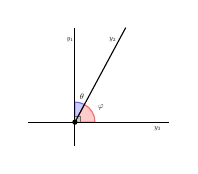
\begin{tikzpicture}[scale=1.5]
\clip(-0.4, -0.2) rectangle (0.8, 0.8);

\node (p) at (\Px, \Py) {};
\node (pp) at (\PPx, \PPy) {};

\filldraw[fill=red!20!white,draw=red!60!white] (0, 0) -- (0.17, 0) arc (\StartAngle:\EndAngle:0.17) -- (0,0);
\filldraw[fill=blue!20!white,draw=blue!60!white] (0, 0) -- (\Cx * 0.17 / \CLength, \Cy * 0.17 / \CLength) arc (\EndAngle:90:0.17) -- (0,0);

\filldraw[fill=black!20!white,draw=black!60!white] (0, 0) 
  -- (\Px * \Scale / \PLength, \Py * \Scale / \PLength)
  -- (\Px * \Scale / \PLength + \PPx * \Scale / \PLength, \Py * \Scale / \PLength + \PPy * \Scale / \PLength)
  -- (\PPx * \Scale / \PLength, \PPy * \Scale / \PLength) -- (0, 0);

\draw (-0.4, 0) -- (0.8, 0);
\draw (0, -0.2) -- (0, 0.8);

\draw (0, 0) -- (\Cx, \Cy);

\node[anchor=north east] at (\Cx, \Cy) {\scalebox{0.25}{$y_2$}};
\node[] at (0.06, 0.22) {\scalebox{0.3}{$\theta$}};
\node[] at (0.22, 0.12) {\scalebox{0.3}{$\varphi$}};


\node[anchor=north] at ($(0.8, 0) + (-0.1, 0.05)$) {\scalebox{0.25}{$y_3$}};
\node[anchor=north east, align=right] at ($(0, 0.8) + (0.07, 0)$) {\scalebox{0.25}{$y_1$}};

\node[circle, fill=black, scale=0.2] at (0, 0) {};
\end{tikzpicture}}
\end{document}   

